The transpose communication pattern reorganizes a given data structure into its transpose representation.
Transpose is a special case of the scatter pattern since it writes its input into a different location in the output memory.

For example it might desirable to transpose a matrix which is represented by a 2D array, laid out in row-major order\footnote{Consecutive elements of a row reside next to each other}.
Transposing such a 2D array will lay out the matrix in column-major order in stead.
An example of transposing a 2D array using the scatter pattern is seen in \autoref{fig:transpose}.
Each thread reads an element from the array but writes its value somewhere scattered in memory according to its stride in the row column transpose.
In the example seen in \autoref{fig:transpose} the stride is three such that each input element with index $i$ will be scattered into "$i\bmod 3$" index in the output array.
\begin{figure}[ht]
	\centering
	\fbox{
		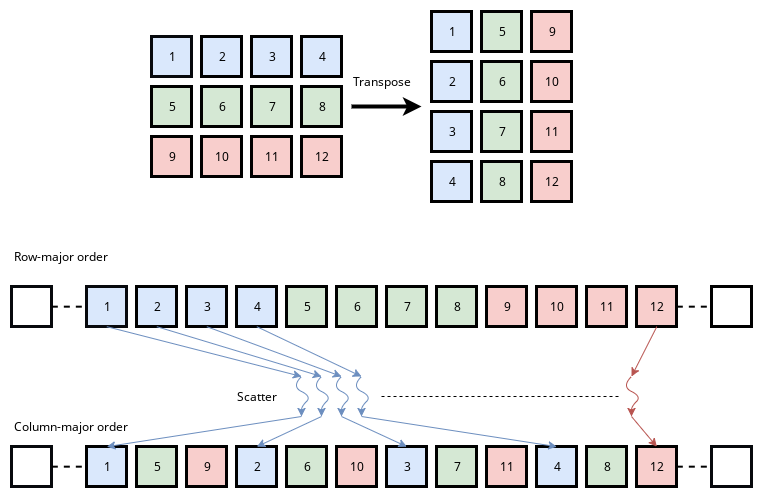
\includegraphics[width=0.6\textwidth]{figs/patterns/parallelTranspose.png}
	}
	\caption{Transpose Pattern}
	\label{fig:transpose}
\end{figure}
A major benefit for using the transpose pattern is that the input structure is reorganized into a more efficient memory structure since CUDA uses coalesced memory transactions when reading from and writing to memory.
The transpose pattern has many use case such as image processing, matrix algebra and more.